\section{Results}

\subsection{Coarse evidence weakens abstention (\clade{})}

\begin{table}[t]
\centering
\small
\setlength{\tabcolsep}{2.9pt}
\begin{tabular}{llcccc}
\toprule
Model & Passage Type & Correct & Wrong & Declines & Prec. \\
\midrule
\multirow{3}{*}{Qwen2.5 7B} & named & 71.7 & 3.8 & 24.5 & 95.0 \\
 & family-only & 26.5 & 18.1 & 55.3 & 59.4 \\
 & silent & 13.8 & 2.5 & 83.8 & 84.6 \\
\midrule
\multirow{3}{*}{OLMo 2 7B} & named & 77.4 & 15.1 & 7.5 & 83.7 \\
 & family-only & 37.2 & 44.7 & 18.1 & 45.5 \\
 & silent & 30.6 & 24.4 & 45.0 & 55.7 \\
\midrule
\multirow{3}{*}{Granite 3.1 8B} & named & 72.6 & 7.5 & 19.8 & 90.6 \\
 & family-only & 30.2 & 26.5 & 43.3 & 53.3 \\
 & silent & 15.0 & 10.0 & 75.0 & 60.0 \\
\midrule
\multirow{3}{*}{Qwen2.5 0.5B} & named & 77.4 & 14.2 & 8.5 & 84.5 \\
 & family-only & 34.4 & 55.8 & 9.8 & 38.1 \\
 & silent & 28.7 & 50.6 & 20.6 & 36.2 \\
\midrule
\multirow{3}{*}{Qwen2.5 14B} & named & 67.9 & 2.8 & 29.2 & 96.0 \\
 & family-only & 24.2 & 17.2 & 58.6 & 58.4 \\
 & silent & 11.9 & 2.5 & 85.6 & 82.6 \\
\bottomrule
\end{tabular}
\caption{Open-book outcomes (\%) on PrimeKG questions where all four distractors come from the answer's MONDO neighborhood (106 named, 215 family-only, and 160 silent questions). Precision is the percentage of correct answers among questions where the model did not abstain.}
\label{tab:outcomes}
\end{table}

\begin{figure}[t]
\centering
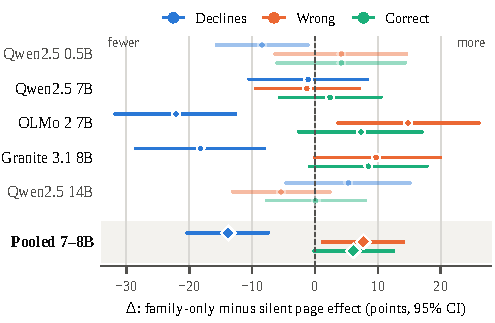
\includegraphics[width=\columnwidth]{figures/fig_forest.pdf}
\caption{Effect of a family-only page relative to a silent page. Each point is $\Delta$ from Eq.~\ref{eq:did} for one outcome, with its 95\% bootstrap CI; points left of zero mean the family-only page lowers that outcome. The pooled row averages the three 7-8B models over 481 questions. Faded rows are models outside the pooled set.}
\label{fig:forest}
\end{figure}

\paragraph{Models abstain less with partial evidence.}
\Cref{tab:outcomes} shows outcomes when the model reads the page. All 7-8B models abstain much less on a family-only page than on a silent page: Qwen2.5-7B from 83.8\% to 55.3\%, OLMo~2 from 45.0\% to 18.1\%, and Granite from 75.0\% to 43.3\%. Many of the extra answers are wrong. Precision, the share of answers that are correct, falls from 83.7-95.0\% on named pages to 45.5-59.4\% on family-only pages.

\paragraph{\clade{} drop comes from context.}
Family-only facts are harder even closed book: they draw more wrong guesses than silent facts in all three 7-8B models (Appendix~D). The page effect in Eq.~\ref{eq:did} removes this difference. Pooled over the models, a silent page raises abstention by $28.5$ points over closed book, but a family-only page raises them by only 14.7 points. The difference $\Delta$ is $-13.8$ points [$-20.3$, $-7.5$], and it stays significant after a Bonferroni correction for three outcomes ($p$=1.1$\times10^{-4}$; \cref{fig:forest}). The freed answers split between wrong answers ($+7.7$ [$1.2$, $14.0$]) and correct ones ($+6.1$ [$-0.1$, $12.4$]). In plain terms, a silent page makes the models stop and say they cannot tell; a family-only page makes them stop much less often, and they guess instead. The drop is significant for OLMo~2 ($-22.1$, $p$=6$\times10^{-6}$), Granite ($-18.2$, $p$=6$\times10^{-4}$) and Qwen2.5-0.5B ($-8.4$, $p$=$0.027$). Qwen2.5-7B shows almost no gap ($-1.1$, $p$=$0.82$). It already declines family-only questions far less often closed book (32.1\% vs.\ 59.4\%), and the page raises its abstention by about the same amount in both groups.

\paragraph{An example.}
For moxifloxacin, PrimeKG lists \emph{Klebsiella pneumonia}, and the page says only that the drug treats pneumonia. All five models pick some bacterial pneumonia with confidence up to 1.00, and none abstains. For lovastatin, OLMo~2 is right closed book but picks a sibling after reading a page that says only \emph{hyperlipidemia} (Appendix~I).

\paragraph{Family size.}
We split the family-only questions into thirds by family size. The drop is large for families of up to 10 members ($-17.3$ [$-26.2$, $-8.2$]) and of 11-20 members ($-18.4$ [$-26.6$, $-10.3$]). It shrinks to $-6.5$ [$-15.7$, $+3.0$] for families above 20 members (\cref{fig:fixes}c). A narrow family makes the page look more answerable.

\subsection{Counterfactual Edits confirm \clade{}}

\begin{figure}[t]
\centering
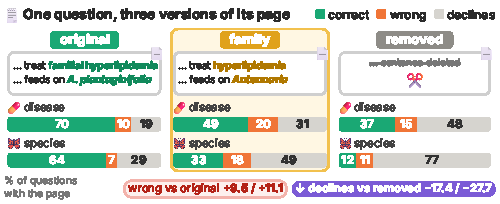
\includegraphics[width=\columnwidth]{figures/fig_example.pdf}
\caption{Page edits on the same questions: PrimeKG (130) and GloBI (255). The \emph{family} edit replaces the answer with its parent; the \emph{removed} edit deletes the sentence. Bars show outcomes with the page (\%), averaged over the 7-8B models.}
\label{fig:edit}
\end{figure}

The edits change only the page (\cref{fig:edit}). Against the original page, the family edit lowers correct answers by 21.0 points and raises wrong answers by 9.5 points, while abstention rises by only 11.5 points. The key comparison is with the removed edit. Keeping the family name instead of deleting the sentence cuts abstention by 17.4 points [$-23.6$, $-11.5$] and raises wrong answers by 5.1 points [$0.5$, $10.3$]. Every model shows this order: from removed to family, abstention falls from 70.0\% to 43.8\% for Qwen2.5-7B, from 56.2\% to 40.8\% for Granite, and from 18.5\% to 7.7\% for OLMo~2. The family name alone suppresses abstention.

\subsection{Three Fixes Fall Short}

\begin{figure*}[t]
\centering
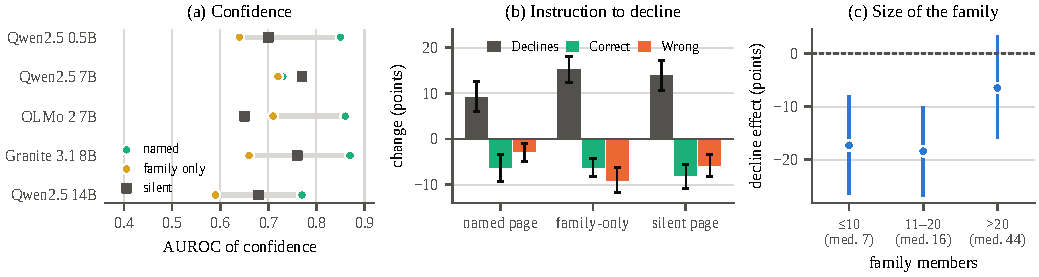
\includegraphics[width=\textwidth]{figures/fig_fixes.pdf}
\caption{Three candidate fixes. (a) Confidence separates correct from wrong answers poorly on family-only pages. (b) An instruction to decline on broad categories raises abstention on every page type, including named pages (pooled 7-8B models, 95\% CIs). (c) The drop in abstention is largest when the family has 20 or fewer members.}
\label{fig:fixes}
\end{figure*}

\paragraph{Confidence does not flag wrong answers.}
AUROC measures how well confidence ranks the correct answers above wrong ones: 1.0 is perfect and 0.5 is chance. On family-only pages it is 0.59-0.72, against 0.73-0.87 on named pages, in every model (\cref{fig:fixes}a). Wrong guesses are confident: their mean probability is 0.77-0.99 in 7-14B models. A threshold that keeps correct answers also keeps most wrong ones.

\paragraph{Scaling does not help.}
Qwen2.5-14B has the best precision on named pages (96.0\%). On family-only pages, precision rises from 38.1\% at 0.5B to 59.4\% at 7B, but then stops: 14B reaches 58.4\%, and it gives 14.7 points more wrong answers than on silent pages ($p$=6$\times10^{-6}$).

\paragraph{Instruction.}
Telling the model not to answer when the page names only a broad category raises abstention by 15.2 points on family-only pages (\cref{fig:fixes}b). It also raises them by 14.0 points on silent pages and 9.1 points on named pages, where it costs 6.3 points of correct answers. Precision on family-only pages stays at 47.9-64.9\%, far below named pages (89.6-94.7\%). The models scores change differently, OLMo~2 abstains far more on all page types, while Granite barely changes (Appendix~F). However, none of these models tells a family name from a specific answer.

\subsection{Second Domain: GloBI}

\begin{table}[t]
\centering
\footnotesize
\setlength{\tabcolsep}{2.6pt}
\begin{tabular}{lrr}
\toprule
Metric & PrimeKG & GloBI \\
\midrule
Questions in pooled set (all-neighbor) & 481 & 833 \\
Abstention page effect, family $-$ silent & $-13.8$ & $-14.3$ \\
Wrong-answer page effect, family $-$ silent & $+7.7$ & $+11.6$ \\
Precision on named passages (\%) & 84--95 & 84--95 \\
Precision on family-only passages (\%) & 45--59 & 22--28 \\
Confidence AUROC on named passages & .73--.87 & .82--.86 \\
Confidence AUROC on family-only passages & .66--.72 & .52--.68 \\
Edit: abstention, family $-$ removed & $-17.4$ & $-27.7$ \\
Edit: wrong answers, family $-$ removed & $+5.1$ & $+6.7$ \\
Edit: correct answers, family $-$ original & $-21.0$ & $-30.8$ \\
\bottomrule
\end{tabular}
\caption{Comparison of biomedical drug--disease facts (PrimeKG with MONDO) and ecological species interactions (GloBI with biological taxonomy) across the three 7--8B models. Effects are reported in percentage points; ranges span individual models. Every difference reported has a 95\% CI excluding zero.}
\label{tab:globi}
\end{table}

Every finding on PrimeKG replicates on species interactions (\cref{tab:globi}). A silent page raises abstention by 12.1 points, but a page that names only the genus or family lowers them by 2.3 points ($\Delta$=$-14.3$, $p$=1.4$\times10^{-9}$). The effect is largest in OLMo~2 ($-31.7$). Here the extra answers are mostly wrong ($+11.6$ wrong, $p$=2.5$\times10^{-8}$; $+2.7$ correct, $p$=$0.09$). Precision on family-only pages falls to 22-28\%, close to the 20\% chance rate, because sibling species are harder to tell apart than sibling diseases. The page edit is even sharper: on 255 questions, keeping the genus name instead of deleting the sentence cuts abstention by 27.7 points [$-32.2$, $-23.5$] and raises wrong answers by 6.7 points (\cref{fig:edit}). \clade{} comes from hierarchical evidence in text, not from medical terms (Appendix~G).

\subsection{Ontology Recovery}

\begin{figure}[t]
\centering
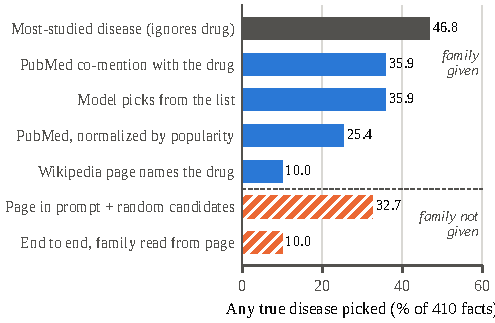
\includegraphics[width=0.9\columnwidth]{figures/fig_recovery.pdf}
\caption{Accuracy of choosing the exact disease for 410 family-only facts. Blue and gray bars choose from the given-family list; hatched bars do not receive the true family.}
\label{fig:recovery}
\end{figure}

\begin{table}[t]
\centering
\small
\setlength{\tabcolsep}{3pt}
\begin{tabular}{@{}lccc@{}}
\toprule
Metric & Given & Page-built & Model-chosen \\
\midrule
Usable lists (of 410) & 410 & 166 & 375 \\
Holds sampled answer & 98.5\% & 19.8\% & 30.0\% \\
Holds any true answer & 99.5\% & 24.6\% & 44.9\% \\
Median list size & 14 & 32 & 12 \\
End-to-end recovery & -- & 10.0\% & 26.8\% \\
\bottomrule
\end{tabular}
\caption{Candidate lists for the 410 family-only facts: given family (oracle), all families on the page (page-built), and the one family Qwen2.5-7B picks from the page (model-chosen). Of the 244 unusable page-built lists, 209 exceed the 64-candidate cap and 35 match no multi-child MONDO family. End-to-end recovery uses the best chooser for each list.}
\label{tab:lists}
\end{table}

\paragraph{List coverage.}
When the right family is given, its MONDO descendants form a list of median 14 candidates. The list holds the sampled answer 98.5\% of the time and some true answer 99.5\% of the time (\cref{tab:lists}).

\paragraph{Finding the family.}
When the family must come from the drug's Wikipedia page, usable lists hold the answer for only 19.8\% of facts. The family is rarely missing; it is buried. A drug article names a median of five MONDO categories, such as comorbidities, side effects and other uses, and their union exceeds 64 candidates for 209 of 410 facts. PubMed makes this worse: coverage drops to 3.7\%. A model does better than string matching. When Qwen2.5-7B reads the page and picks one of the families it names, the chosen list holds the answer for 30.0\% of facts (44.9\% for any true answer), above the first-mentioned family (25.1\%) and a random one (13.9\%). The ceiling is 50.0\%: for half of the facts, the right family is not among the usable families on the page.

\paragraph{Choosing a member.}
Within the given-family list (\cref{fig:recovery}), Qwen2.5-7B alone reaches 35.9\% (32.4\% with the page in the prompt), and raw PubMed co-mentions also reach 35.9\%. Evidence first, with the model as a fallback, reaches 41.7\%. Yet the best chooser ignores the drug: picking the disease with the most PubMed abstracts reaches 46.8\%. When we divide co-mentions by each disease's abstract count, accuracy drops from 35.9\% to 25.4\%, so co-mentions work mainly because common diseases are studied more.

\paragraph{Errors and end-to-end recovery.}
Most misses pick a better-studied sibling, such as \emph{ovarian carcinoma} instead of \emph{malignant germ cell tumor of ovary} for carboplatin, or a valid use missing from PrimeKG, so strict graph scoring understates accuracy (Appendix~H). Without the given family, page-built lists recover the answer for 10.0\% of facts with Wikipedia and 1.5\% with PubMed added; model-chosen lists recover 26.8\% (\cref{tab:lists}).
